\subsubsubsubsection{House}
\begin{figure}[h]
\centering
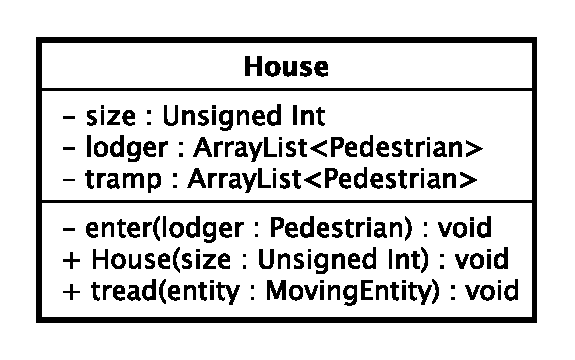
\includegraphics[scale=0.6,keepaspectratio]{images/solution/house.eps}
\caption{\pReactiveComponentStretchDecoration::House}
\label{fig:sd-app-house}
\end{figure}
\FloatBarrier
\begin{itemize}
  \item \textbf{\descr} \\
    It represents a house which can host several pedestrians.
  \item \textbf{\attrs}
  \begin{itemize}
    \item \texttt{size: Unsigned Int} \\
The maximum number of pedestrians that can be hosted into the house.
    \item \texttt{lodgers: Collection<Pedestrian>} \\
The collection of pedestrians that are currently hosted into the house.
  \end{itemize}
  \item \textbf{\ops}
  \begin{itemize} 
   \item[+] \texttt{House(size: Unsigned Int)} \\
Creates a house specifying its maximum number of lodgers.
    \item \texttt{enter(pedestrian: Pedestrian)} \\
The house is not full and the pedestrian become a lodger.   
\item[+] \texttt{tread(entity: MovingEntity)} \\
Implements the permanence of the pedestrian into the house. First the house notifies the moving entity that there is a building in the current stretch. After receiving a reply, the house checks the entities specified in the reply message. If the house is not full it invokes enter, otherwise the pedestrian is forced to switch to the next step of its route. At the end the house register itself for a timeout notification.
  \end{itemize}
\end{itemize}
